% Options for packages loaded elsewhere
% Options for packages loaded elsewhere
\PassOptionsToPackage{unicode}{hyperref}
\PassOptionsToPackage{hyphens}{url}
\PassOptionsToPackage{dvipsnames,svgnames,x11names}{xcolor}
%
\documentclass[
  letterpaper,
  DIV=11,
  numbers=noendperiod]{scrartcl}
\usepackage{xcolor}
\usepackage{amsmath,amssymb}
\setcounter{secnumdepth}{-\maxdimen} % remove section numbering
\usepackage{iftex}
\ifPDFTeX
  \usepackage[T1]{fontenc}
  \usepackage[utf8]{inputenc}
  \usepackage{textcomp} % provide euro and other symbols
\else % if luatex or xetex
  \usepackage{unicode-math} % this also loads fontspec
  \defaultfontfeatures{Scale=MatchLowercase}
  \defaultfontfeatures[\rmfamily]{Ligatures=TeX,Scale=1}
\fi
\usepackage{lmodern}
\ifPDFTeX\else
  % xetex/luatex font selection
\fi
% Use upquote if available, for straight quotes in verbatim environments
\IfFileExists{upquote.sty}{\usepackage{upquote}}{}
\IfFileExists{microtype.sty}{% use microtype if available
  \usepackage[]{microtype}
  \UseMicrotypeSet[protrusion]{basicmath} % disable protrusion for tt fonts
}{}
\makeatletter
\@ifundefined{KOMAClassName}{% if non-KOMA class
  \IfFileExists{parskip.sty}{%
    \usepackage{parskip}
  }{% else
    \setlength{\parindent}{0pt}
    \setlength{\parskip}{6pt plus 2pt minus 1pt}}
}{% if KOMA class
  \KOMAoptions{parskip=half}}
\makeatother
% Make \paragraph and \subparagraph free-standing
\makeatletter
\ifx\paragraph\undefined\else
  \let\oldparagraph\paragraph
  \renewcommand{\paragraph}{
    \@ifstar
      \xxxParagraphStar
      \xxxParagraphNoStar
  }
  \newcommand{\xxxParagraphStar}[1]{\oldparagraph*{#1}\mbox{}}
  \newcommand{\xxxParagraphNoStar}[1]{\oldparagraph{#1}\mbox{}}
\fi
\ifx\subparagraph\undefined\else
  \let\oldsubparagraph\subparagraph
  \renewcommand{\subparagraph}{
    \@ifstar
      \xxxSubParagraphStar
      \xxxSubParagraphNoStar
  }
  \newcommand{\xxxSubParagraphStar}[1]{\oldsubparagraph*{#1}\mbox{}}
  \newcommand{\xxxSubParagraphNoStar}[1]{\oldsubparagraph{#1}\mbox{}}
\fi
\makeatother


\usepackage{longtable,booktabs,array}
\usepackage{calc} % for calculating minipage widths
% Correct order of tables after \paragraph or \subparagraph
\usepackage{etoolbox}
\makeatletter
\patchcmd\longtable{\par}{\if@noskipsec\mbox{}\fi\par}{}{}
\makeatother
% Allow footnotes in longtable head/foot
\IfFileExists{footnotehyper.sty}{\usepackage{footnotehyper}}{\usepackage{footnote}}
\makesavenoteenv{longtable}
\usepackage{graphicx}
\makeatletter
\newsavebox\pandoc@box
\newcommand*\pandocbounded[1]{% scales image to fit in text height/width
  \sbox\pandoc@box{#1}%
  \Gscale@div\@tempa{\textheight}{\dimexpr\ht\pandoc@box+\dp\pandoc@box\relax}%
  \Gscale@div\@tempb{\linewidth}{\wd\pandoc@box}%
  \ifdim\@tempb\p@<\@tempa\p@\let\@tempa\@tempb\fi% select the smaller of both
  \ifdim\@tempa\p@<\p@\scalebox{\@tempa}{\usebox\pandoc@box}%
  \else\usebox{\pandoc@box}%
  \fi%
}
% Set default figure placement to htbp
\def\fps@figure{htbp}
\makeatother





\setlength{\emergencystretch}{3em} % prevent overfull lines

\providecommand{\tightlist}{%
  \setlength{\itemsep}{0pt}\setlength{\parskip}{0pt}}



 


\KOMAoption{captions}{tableheading}
\makeatletter
\@ifpackageloaded{caption}{}{\usepackage{caption}}
\AtBeginDocument{%
\ifdefined\contentsname
  \renewcommand*\contentsname{Table of contents}
\else
  \newcommand\contentsname{Table of contents}
\fi
\ifdefined\listfigurename
  \renewcommand*\listfigurename{List of Figures}
\else
  \newcommand\listfigurename{List of Figures}
\fi
\ifdefined\listtablename
  \renewcommand*\listtablename{List of Tables}
\else
  \newcommand\listtablename{List of Tables}
\fi
\ifdefined\figurename
  \renewcommand*\figurename{Figure}
\else
  \newcommand\figurename{Figure}
\fi
\ifdefined\tablename
  \renewcommand*\tablename{Table}
\else
  \newcommand\tablename{Table}
\fi
}
\@ifpackageloaded{float}{}{\usepackage{float}}
\floatstyle{ruled}
\@ifundefined{c@chapter}{\newfloat{codelisting}{h}{lop}}{\newfloat{codelisting}{h}{lop}[chapter]}
\floatname{codelisting}{Listing}
\newcommand*\listoflistings{\listof{codelisting}{List of Listings}}
\makeatother
\makeatletter
\makeatother
\makeatletter
\@ifpackageloaded{caption}{}{\usepackage{caption}}
\@ifpackageloaded{subcaption}{}{\usepackage{subcaption}}
\makeatother
\usepackage{bookmark}
\IfFileExists{xurl.sty}{\usepackage{xurl}}{} % add URL line breaks if available
\urlstyle{same}
\hypersetup{
  pdftitle={Introducción a las GPUs Nvidia},
  colorlinks=true,
  linkcolor={blue},
  filecolor={Maroon},
  citecolor={Blue},
  urlcolor={Blue},
  pdfcreator={LaTeX via pandoc}}


\title{Introducción a las GPUs Nvidia}
\author{}
\date{}
\begin{document}
\maketitle


\section{Introducción a la arquitectura de una
GPU}\label{introducciuxf3n-a-la-arquitectura-de-una-gpu}

Para desbloquear el potencial completo de una GPU, es necesario conocer
la arquitectura del Hardware. El enfoque de este documento tiene de
propuesta conocer la Arquitectura de Hardware de las GPUs.

\subsection{GPU vs CPU}\label{gpu-vs-cpu}

\begin{longtable}[]{@{}
  >{\raggedright\arraybackslash}p{(\linewidth - 2\tabcolsep) * \real{0.4667}}
  >{\raggedright\arraybackslash}p{(\linewidth - 2\tabcolsep) * \real{0.5333}}@{}}
\toprule\noalign{}
\begin{minipage}[b]{\linewidth}\raggedright
CPU
\end{minipage} & \begin{minipage}[b]{\linewidth}\raggedright
GPU
\end{minipage} \\
\midrule\noalign{}
\endhead
\bottomrule\noalign{}
\endlastfoot
ALU con gran capacidad & Miles de pequeñas ALUs (Cores) \\
Cache de memoria grande por ALU & Caches pequeñas por core \\
Ideal para aplicaciones secuenciales & Ideal para aplicaciones
paralelizables \\
\end{longtable}

\begin{figure}[H]

{\centering \pandocbounded{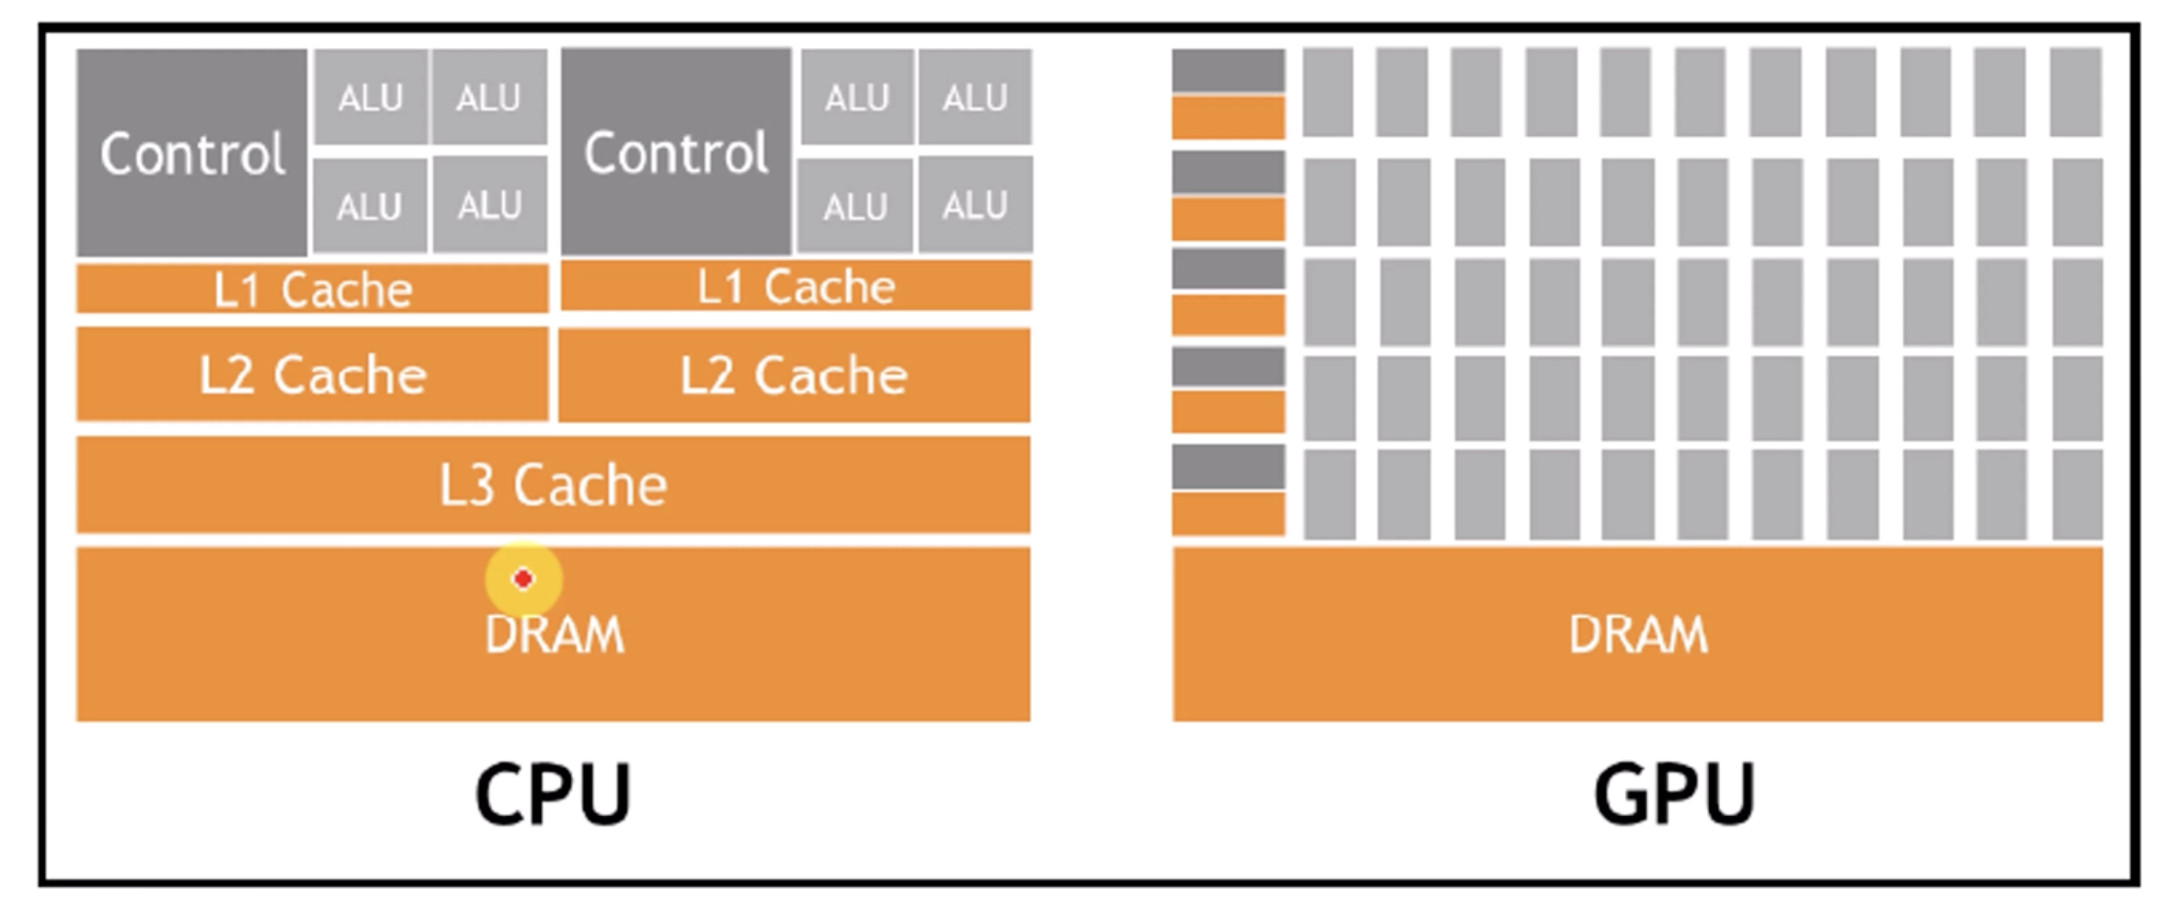
\includegraphics[keepaspectratio]{resources/GPUsVSCPUarch.png}}

}

\caption{Diagrama de arquitectura de una CPU vs GPU}

\end{figure}%

\subsection{GPU hardware en general}\label{gpu-hardware-en-general}

\begin{itemize}
\tightlist
\item
  \emph{Streaming Multiprocessor(SM)}
\item
  \emph{Niveles de memoria (L2 cache y Device Global Memory) }
\item
  Scheduler and Dispatcher
\end{itemize}

Dentro del Streaming Multiprocessor se encuentrar una gran cantidad de
cores, diseñador para tareas específicas. Algunos cores estan dedicados
para ejecutar operaciones de punto flotante y otro para ejecutar
operaciones con enteros.

\begin{figure}[H]

{\centering \pandocbounded{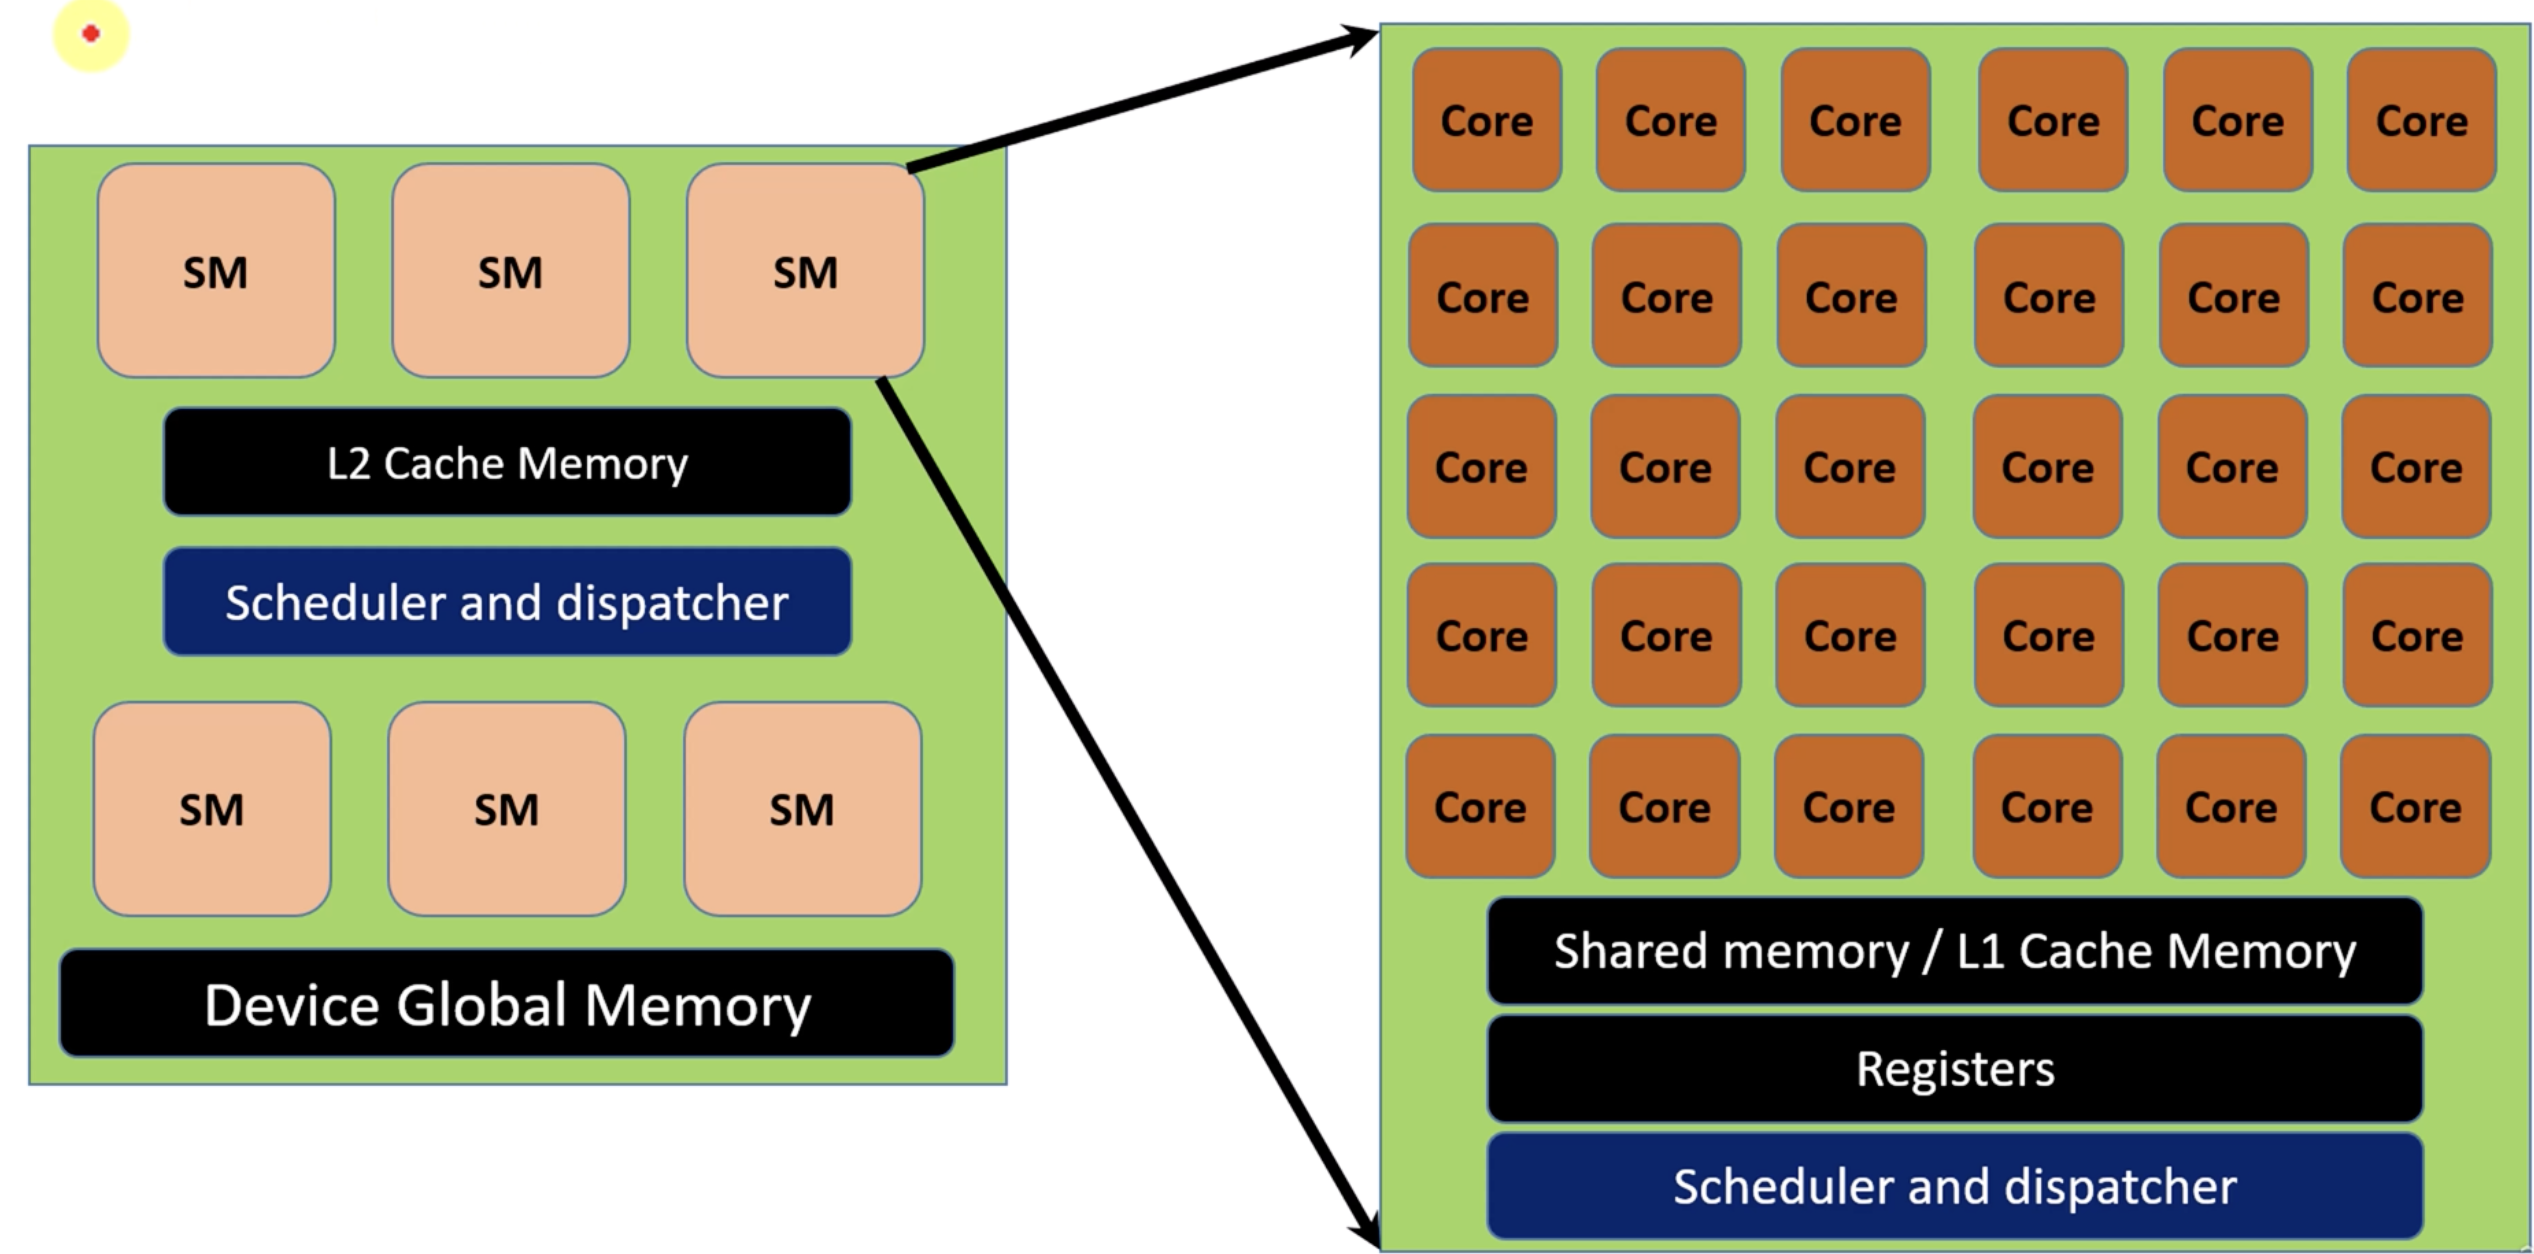
\includegraphics[keepaspectratio]{resources/GPUArch.png}}

}

\caption{Arquitecutra general de un GPU}

\end{figure}%

\subsection{GPU arquitectura}\label{gpu-arquitectura}

\begin{itemize}
\tightlist
\item
  \textbf{Definición:} Diseño y estructura
\item
  La arquitectura determina la eficiencia y performance.
\item
  Nombre de las Arquitecturas (Nombres de científicos).
\end{itemize}

\subsection{Categorias}\label{categorias}

Existen dos categorías

\subsubsection{Estandar}\label{estandar}

Para usuarios normales, comprende las generaciones:

\begin{itemize}
\tightlist
\item
  \textbf{Tegra}
\item
  \textbf{Geforce}
\item
  \textbf{Quadro}
\end{itemize}

Por ejemplo RTX xxxx (3090)

\subsubsection{HPC GPUs}\label{hpc-gpus}

Computo de alto redimiento.

\begin{itemize}
\tightlist
\item
  \textbf{Tesla}
\end{itemize}

Por ejemplo H100, A100, V100.

El término \textbf{Generación} se refiere al uso específico de la GPU,
en cambio el término \textbf{Arquitectura} se refiere al diseño del Chip
de las capacidades de la GPU, una arquitectura puede contener más de una
generación.

\subsection{Principales parámetros que impactan el performance en
GPUs}\label{principales-paruxe1metros-que-impactan-el-performance-en-gpus}

\begin{itemize}
\tightlist
\item
  Ancho de banda de Memoria (memory speed + bus width).
\item
  Rendimiento de TFlops. (Numero de cores + Velocidad).
\item
  Nuevas funcionalidades. (Soporte de nuevos tipos de datos - tensor
  cores).
\end{itemize}

\subsection{Memory Bandwidth}\label{memory-bandwidth}

Se refiere a cuanta información puede procesar la memoria por segundo
(GBs)

En la imagene podemos observar que ambas arquitecturas poseen el mismo
numero de cores, pero la memoria dos tiene cuatro veces mas capacidad de
realizar las operaciones de lectura y escritura que la memoria uno, por
lo que si los cuatros cores requieren leer 32 bits una realizara la
operación en un segundo mientras que la que solo su memory bandwidth es
de 32 bits por segundo requiere de 4 segundos.

\begin{figure}[H]

{\centering \pandocbounded{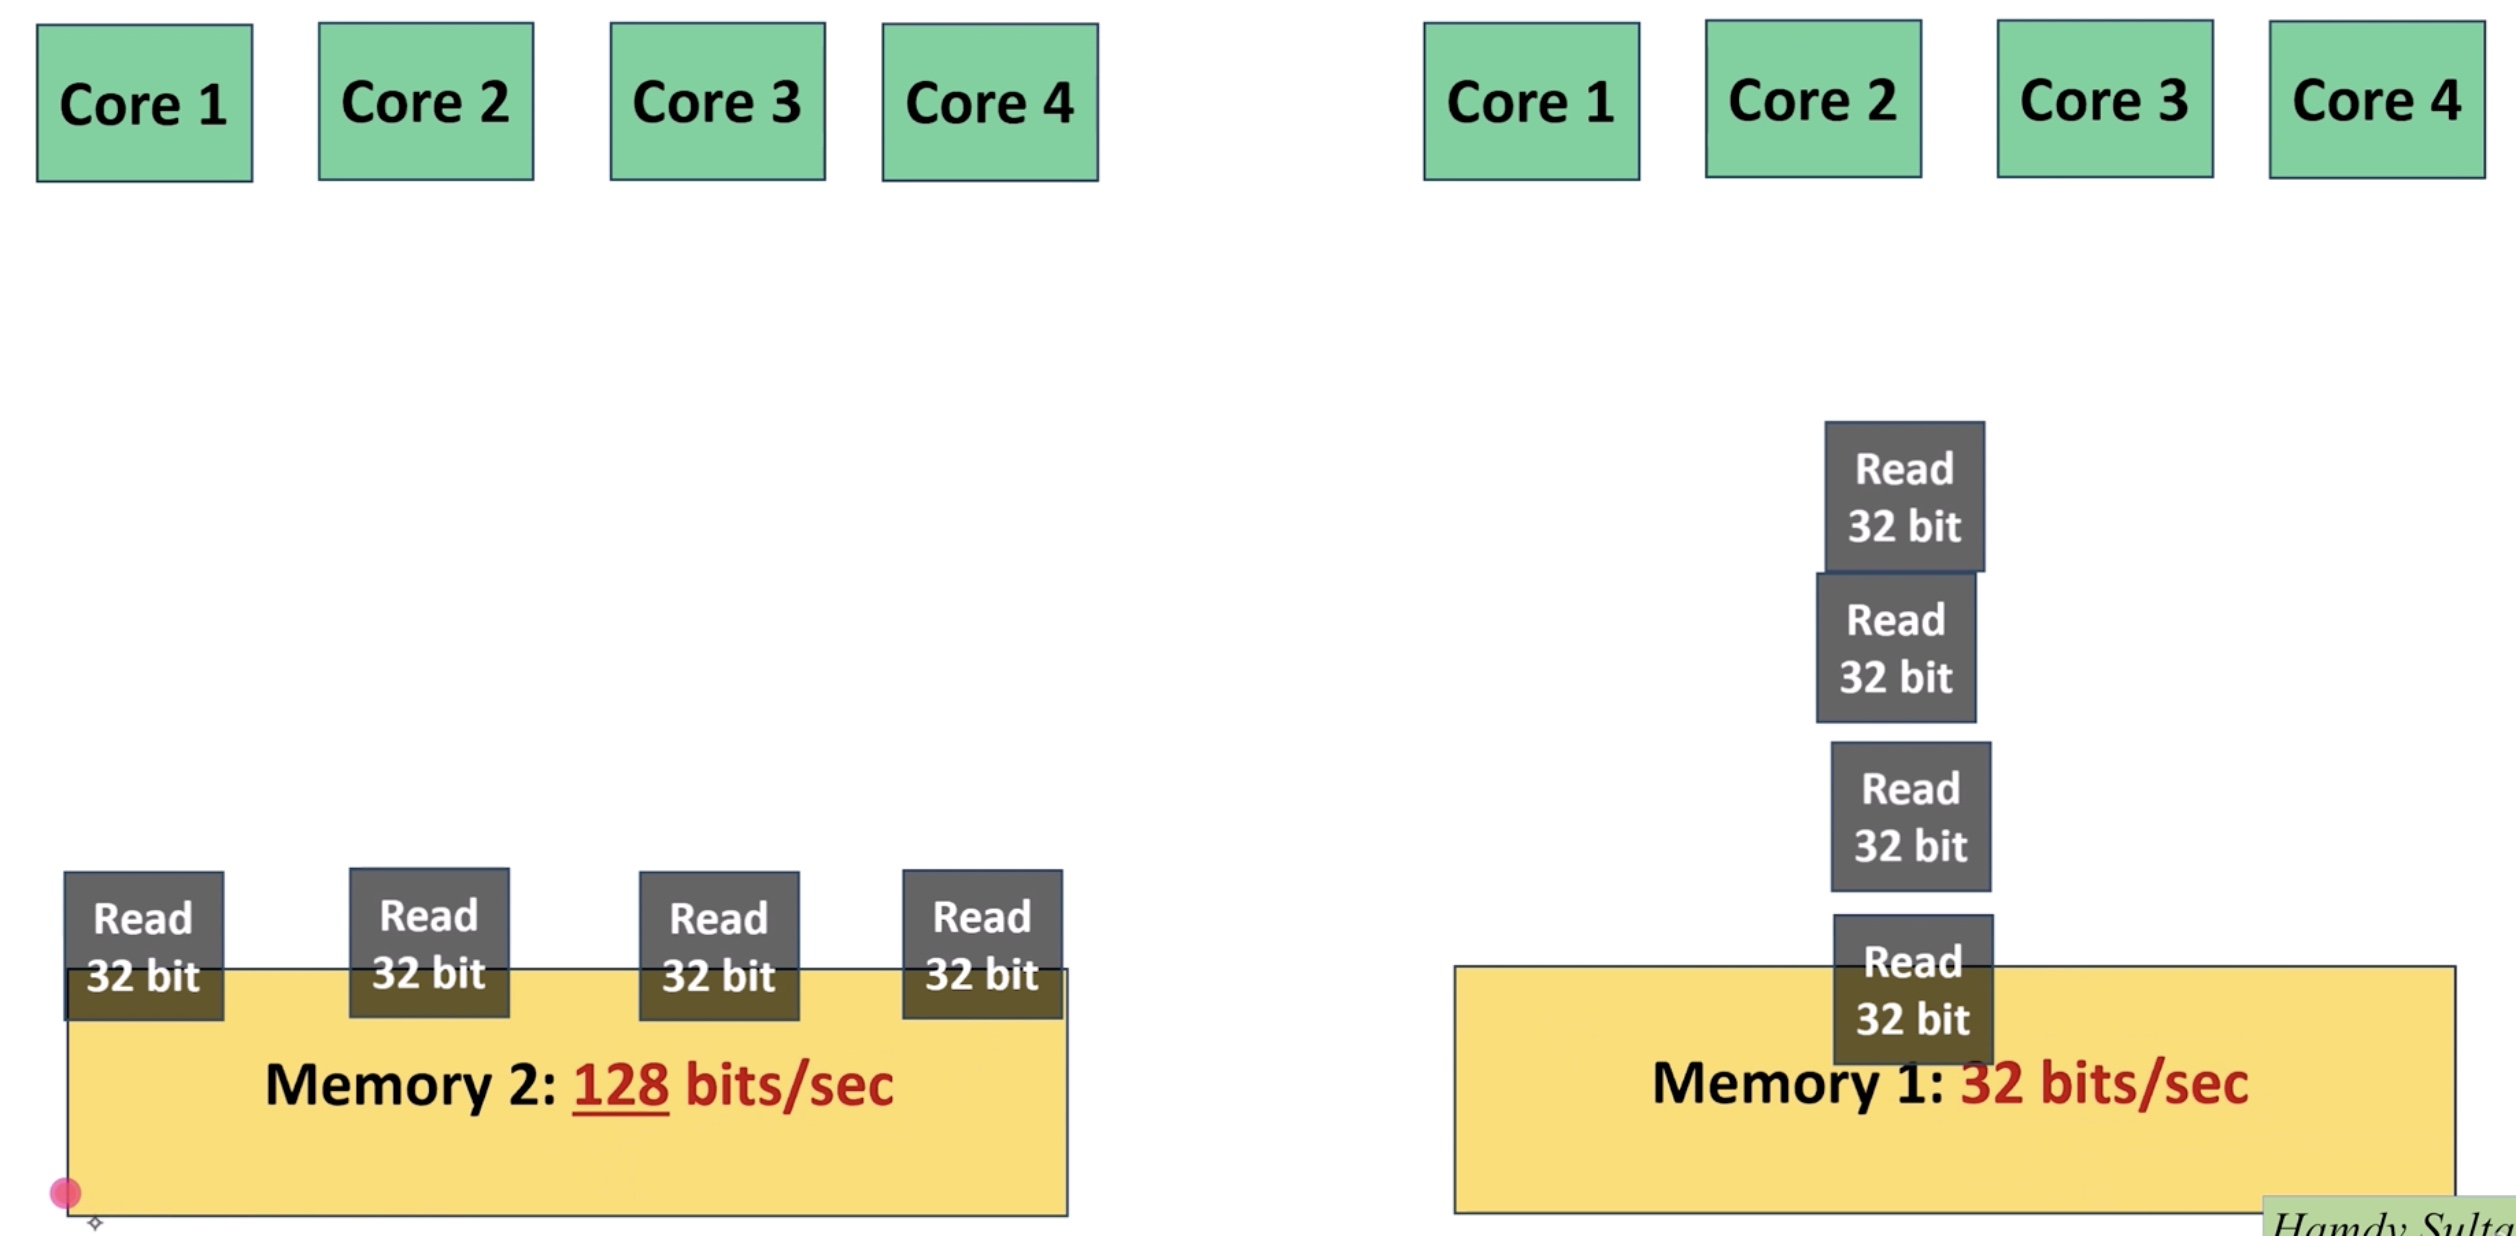
\includegraphics[keepaspectratio]{resources/MemoryBandWidth.jpeg}}

}

\caption{Memory Bandwidth}

\end{figure}%

\subsection{Rendimiento de TFlops}\label{rendimiento-de-tflops}

El rendimiento en TFlop se refiere al número total de instrucciones por
segundo que son ejecutadas por el GPU completo.

Un mayor número de cores se traduce en incrementar la capacidad de
procesamiento paralelo. Aunque un mayor número de cores no implica que
se realice más rapido un tarea ya que hay otro factor importante
\textbf{core speed}.

\subsection{CUDA Compiler (nvcc)}\label{cuda-compiler-nvcc}

El compilador nvcc es la clave para transformar código de alto nivel en
una forma que la GPU entiende. Convierte aplicaciones CUDA en PTX Code
que es compatible con varias arquitecturas de GPU.

\subsection{Librerias de CUDA}\label{librerias-de-cuda}

Estás libreras estan diseñadas para optimizar las operaciones
significativamente.

\begin{itemize}
\tightlist
\item
  \textbf{cuBLAS:} GPU-accecelerated Basic Linear-Algebra subprograms.
\item
  \textbf{cuFFT:} Fast Fourier Transform library GPUs.
\item
  \textbf{cuRAND:} Random Numero Generation library.
\item
  \textbf{cuDNN:} Deep Neural Network libray used for deep learning
  applicactions.
\end{itemize}

\subsection{CUDA Runtime and Driver
APIs}\label{cuda-runtime-and-driver-apis}

Provee interfaces de bajo y alto nivel para manejar, dispositivos,
memoria y ejecución del programa en el GPU.

\begin{itemize}
\item
  \textbf{cudaMalloc():} Para transferencia de datos entre el CPU y el
  GPU, usamos esta función. De esta forma nosotros disponemos de la
  memoria del GPU.
\item
  \textbf{cudaMemcpy():} Utilizada para copiar información entre el host
  (CPU) y la GPU, ya sea de la GPU a CPU o de la CPU a la GPU.
\end{itemize}

\section{Herramientas de NVIDIA para DEBUGGING y Performance
Analysis:}\label{herramientas-de-nvidia-para-debugging-y-performance-analysis}

EL toolkit de NVIDIA incluye herramientas como :

\begin{itemize}
\item
  \textbf{NVIDIA Nsight System:} For system-wide performance analysis.
\item
  \textbf{NVIDIA Nsight Compute:} For detailed CUDA kernel profiling and
  analysis.
\item
  \textbf{CUDA-GDB:} The NVIDIA tool for debugging CUDA applications on
  linux and Mac OS.
\item
  \textbf{CUDA-MEMCHECK:} Tool to detect and diagnose memory errors in
  CUDA applications.
\end{itemize}

Repositorio del curso de CUDA:\\
https://github.com/hamdysoltan/CUDA\_Course

```Python print(``hola mundo'')




\end{document}
